% 1. novel approach, why? protection goals and performance → security and efficiency
% 2. what precisely was done at the TUD chair → say that their research proved the potential of NC and that's why we persue it here again
% 3. NC provides no confidentiality/integrity guarantees → we implement encryption+authentication
% 3.1 Availability only partially adressed
% 3.2 recall NoC architecture → this is implemented in the network interfaces
% 4. Different variants envisioned (3 methods) + comparison with uncoded variant where applicable
% 5. Multiple paths focus → why multiple paths in the first place? → chance to avoid compromised routers, still have enough flits
%    thanks to NC
% 6. Routing strategies: deterministic vs. non-deterministic routing → XY, smart random XY, ROMM+XY, ROMM+srXY
% 7. Attacker/Threat model
% 8. Evaluation
% Always refer to the chapters that explain this in detail
In this thesis, a novel approach for securing the communications in a \gls{noc} is pursued. The goal is to design and implement a protocol that
remedies both accidental and malicious modifications to the transmitted data as much as possible while meeting the performance requirements of a \gls{noc} (cf. Section
\ref{sec:networkonchipfun}). In this thesis, a scheme is envisioned and investigated that attempts to satisfy these ambitions by combining encryption
and authentication techniques with network coding and multipath routing.

In the next section, the necessity of such security measures is corroborated. Subsequently, the attacker model that the schemes explored in this
thesis aim to defend against is illustrated. Afterwards, an overview of the utilized techniques and how they are
integrated into a \gls{noc} architecture is given. Furthermore, different variants of the envisioned protocol are introduced. Finally, the
methodology for evaluating the design through in-depth simulations is presented.

\section{Necessity Of Security Measures}\label{sec:necessityofsecurity}
In Section \ref{sec:nocsecurity}, it was shown that attacks specifically tailored for \gls{noc} architectures are feasible and practical. In
particular, hardware trojans pose a potent threat to \glspl{mpsoc} that incorporate \glspl{noc} as their communication backbone. Pure software attacks
originating from a processing element are feasible as well \cites(e.g.)(){biswas15routerattack}{kocher04embeddedsecurity}, but will not be considered
during this thesis. % TODO: schöner formulieren?

There are a number of possible infection vectors that adversaries may try to exploit in order to covertly introduce a hardware trojan into a \gls{noc}
implemented in an \gls{mpsoc}\footnote{Theoretically, the aforementioned infection vectors are not specific to \glspl{mpsoc} and \glspl{noc}, but
this is the relevant constellation for the scope of this thesis.}. One such vector is the integration of third party \gls{ip}\footnote{An example of
this is the Arteris FlexNoC interconnect, which is used by \enquote{four out of the top five Chinese fabless semiconductor OEM companies}
\cite[2]{ancajas14fortnocs}.}, which has become increasingly popular due to cost efficiency and growing circuit complexity
\cites[1]{ancajas14fortnocs}[2]{bhunia14hardwaretrojans}. These third parties may have an interest in equipping their \gls{ip} with a hardware trojan,
and their trustworthiness is usually not guaranteed \cite[3]{sethumadhavan15trustworthyhardware}.
Another practical scenario is a rogue employee \enquote{subvert[ing] the design} \cite[3]{sethumadhavan15trustworthyhardware} of his
company's product. For example, a hardware designer \enquote{participating in the design process} \cite[3]{sethumadhavan15trustworthyhardware} may
secretly introduce a hardware trojan at one point. 

The illustrated scenarios are not an exhaustive list of infection vectors, but they clearly corroborate the need for countermeasures. The ones pursued
for this thesis will be presented in the following sections.

\section{Attacker Model}
For the experiments in this thesis, the threat of a compromised \gls{noc} is explored. More specifically, the routers may be infected by a hardware
trojan, while the network interfaces are considered trustworthy. This is the same attacker model as the one used by \citeauthor{moriam18activeattackers}
\cite{moriam18activeattackers} in the work preceding this thesis. It is based on the assumption that routers and their interconnections are
more likely to be obtained from third party vendors than network interfaces, making them more susceptible to concealed hardware trojans. The reasoning
for this is that \enquote{routers have a deterministic functionality} \cite[2]{moriam18activeattackers} that does not depend on the peculiarities of
a specific system. In contrast, network interfaces often contain product-specific logic and are thus \enquote{rather developed in house and under
control} \cite[2]{moriam18activeattackers}, eliminating the attack vector of third party \gls{ip}. This model is visualized in Figure
\vref{fig:noctrustboundaries}.

\begin{figure}
    \centering
    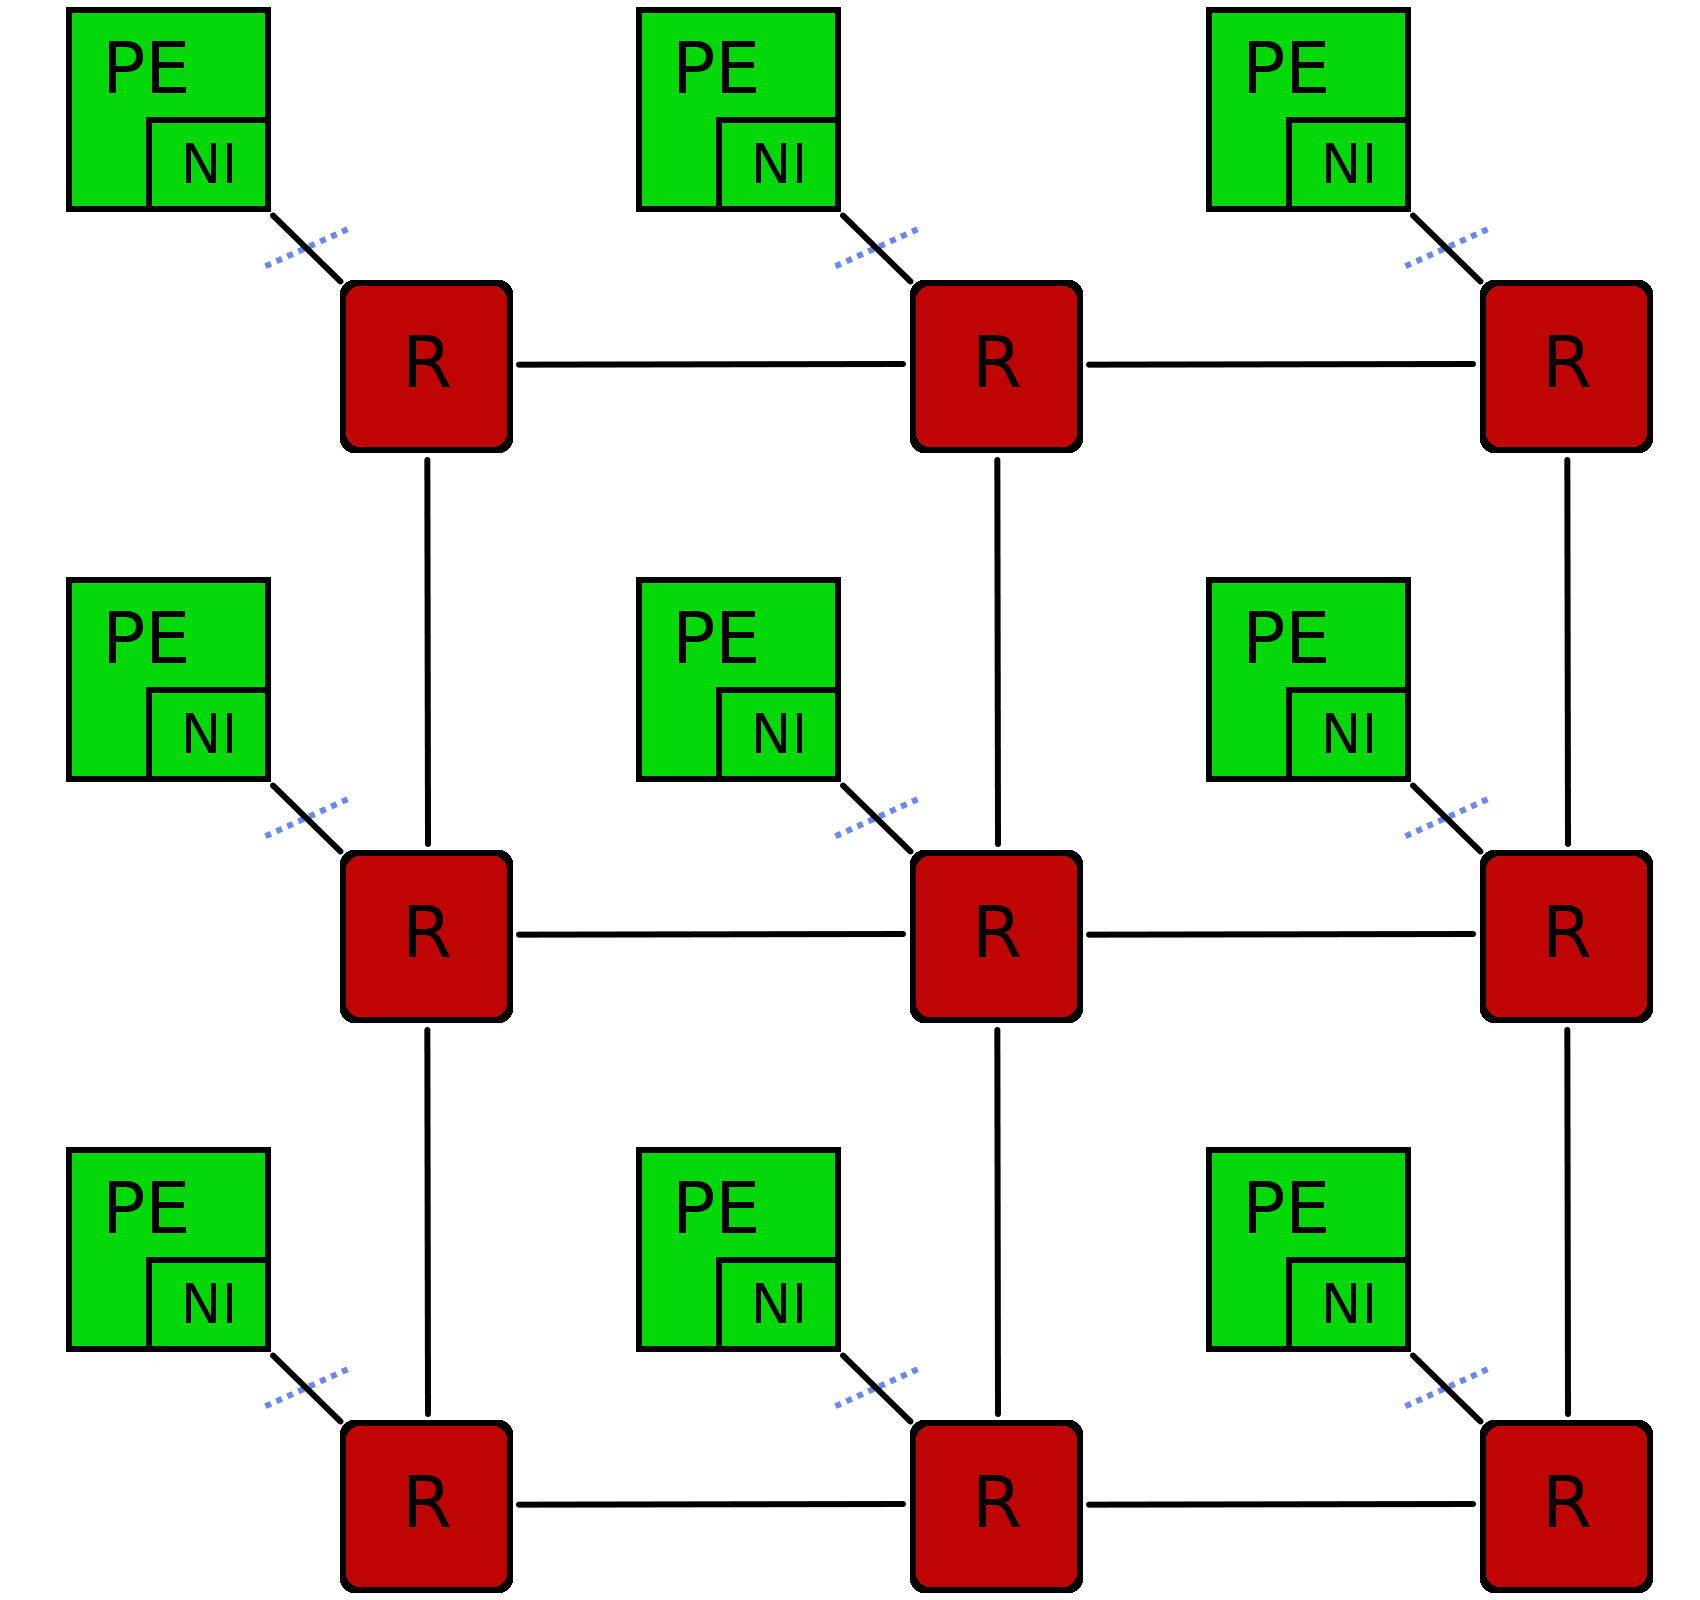
\includegraphics[width=0.6\textwidth]{noc-trust-boundaries}
    \caption[Trust boundaries in a NoC]{Visualization of the trusted and untrusted hardware components in a NoC. The processing elements and network
    interfaces, which are assumed to be trusted, are marked green. The network itself, which is comprised of the routers and their interconnections,
    is not trustworthy and thus marked red. The dotted lines at the local connections mark the trust boundaries.}
    \label{fig:noctrustboundaries}
\end{figure}

\section{Encryption And Authentication}
The intent of integrating encryption and authentication is to provide confidentiality and integrity to communications passing through a \gls{noc}. To
implement this, a new network interface design is proposed. Since all flits that enter the \gls{noc} must pass through a network interface, this is the
ideal location to implement cryptographic protection. In the proposed design, it encrypts all outgoing flits, which can only be decrypted by the
receiver. In addition, a \gls{mac} is computed that is sent together with the encrypted flits. On the receiver side, the flits are decrypted and the
\gls{mac} is verified. This scheme is illustrated in Figure \vref{fig:nocflitencauth} and further explained in Section (insert ref here).

\begin{figure}
    \centering
    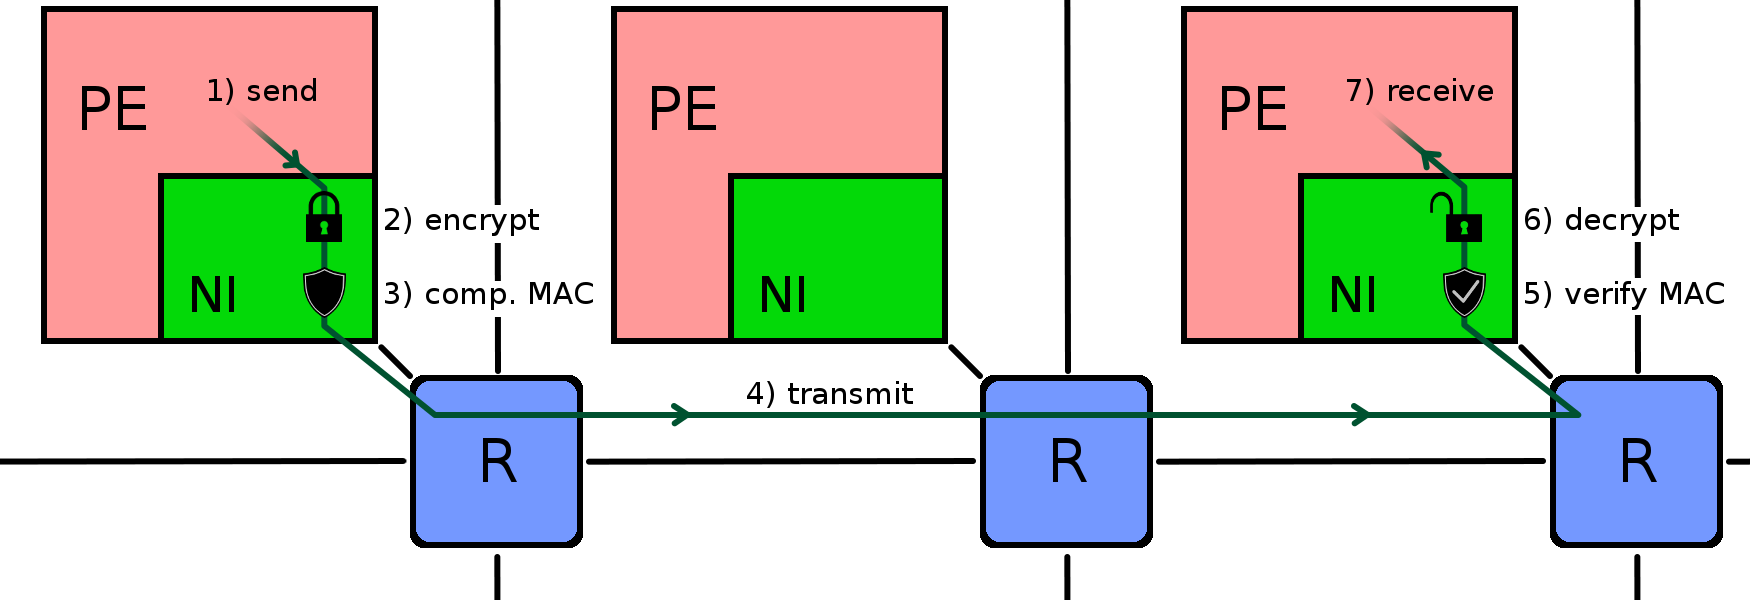
\includegraphics[width=\textwidth]{noc-message-enc-auth}
    \caption[Flit through NoC with encryption and authentication]{Example of a flit being transmitted through a NoC. After a processing element sends a flit (1),
    encryption is applied (2) and a MAC is computed (3) in the sender's network interface. The encrypted flit and the MAC are then routed to the
    destination (4). There, the receiver's network interface verifies the MAC (5) and decrypts the flit (6). Finally, the flit is passed to the
    receiving processing element (7).} % TODO: state that this is "method 1 uncoded"?
    \label{fig:nocflitencauth}
\end{figure}

The ciphers that were investigated for this purpose use symmetric cryptography, as this allows for efficient cryptographic computations.
In addition, the produced \glspl{mac} are short enough to fit into a single flit. However, their usage implies that each pair of
sender and receiver needs to possess a shared secret key. To obtain or renegotiate such a key in a secure manner, a key exchange algorithm is required.
As this goes beyond the scope of this thesis, each pair of sender and receiver is assumed to own a shared secret key. The alternative, asymmetric
cryptography, is not considered, since it \enquote{implies a high computational effort} \cite[3]{moriam18activeattackers}. Additionally, this class of
algorithms produces signatures instead of \glspl{mac}, which are \enquote{too long to be included in a flit} \cite[3]{moriam18activeattackers}.

\section{Random Linear Network Coding}
While network coding provides robustness against sporadic flit loss, it does not provide any guarantees on the integrity of flits.

\section{Multipath Routing}

\section{Protocol Variants}

\section{Evaluation Approach}
First: fix the hyperparameters, then experiments with the remaining parameters and protocol variants
\subsection{Simulation}



As mentioned in Chapter \ref{ch:introduction}, this thesis aims to pursue a novel approach for providing secure and efficient communication in
\glspl{noc}.

This thesis follows up on previous work done at the \thechair. In 2015, the effect of network coding
on communications in a partially compromised \gls{noc} was evaluated and discussed. Now, the emphasis lies on combining network coding with
cryptographic measures to fulfill the desired protection goals (see Section (vref to fundamentals)). % TODO: move this to introduction?
% Mention that NoC will be simulated

In this thesis, the suitability of encryption and authentication techniques to provide confidentiality and integrity is examined. However, the
constraints imposed by the \gls{noc} environment (cf. Section \ref{sec:networkonchipfun}) make this a challenging task.

This thesis: no hardware synthesis, use software simulation. Focus on malicious flit modification (→ attacker model) rather than DoS attacks. Our
model assumes that the NoC routers and links may be compromised and thus relies on the NIs for the security measures → no effective protection
against bandwidth depletion, but this is not the goal.
Deterministic vs. static routing? No security zones or division into secure/non-secure zones/cores.
